\section{Moving from sequence to atomic structure scenario}

\subsubsection*{Downloading the atomic structure}
  
  Once identified the \iii{template} that we are going to use as structural skeleton of our sequence, we import it into \scipion with the protocol \scommand{import atomic structure} (Appendix \ref{app:importAtomicStructure},  \ffigure{fig:import_atomic_structure} (1)). Select the option for importing the atomic structure from ID (2), write the \ttt{PDB} accession code (3) and execute the protocol (4). You can visualize the imported structure (5) in $Chimera$ (\ffigure{fig:chimera_visualization_structure}). By selecting chain \ttt{A} in the $Chimera$ upper menu (1) you can distinguish the \ttt{Hgb} $\alpha$ subunit (2).
  
  \begin{figure}[H]
  \centering 
  \captionsetup{width=.7\linewidth} 
  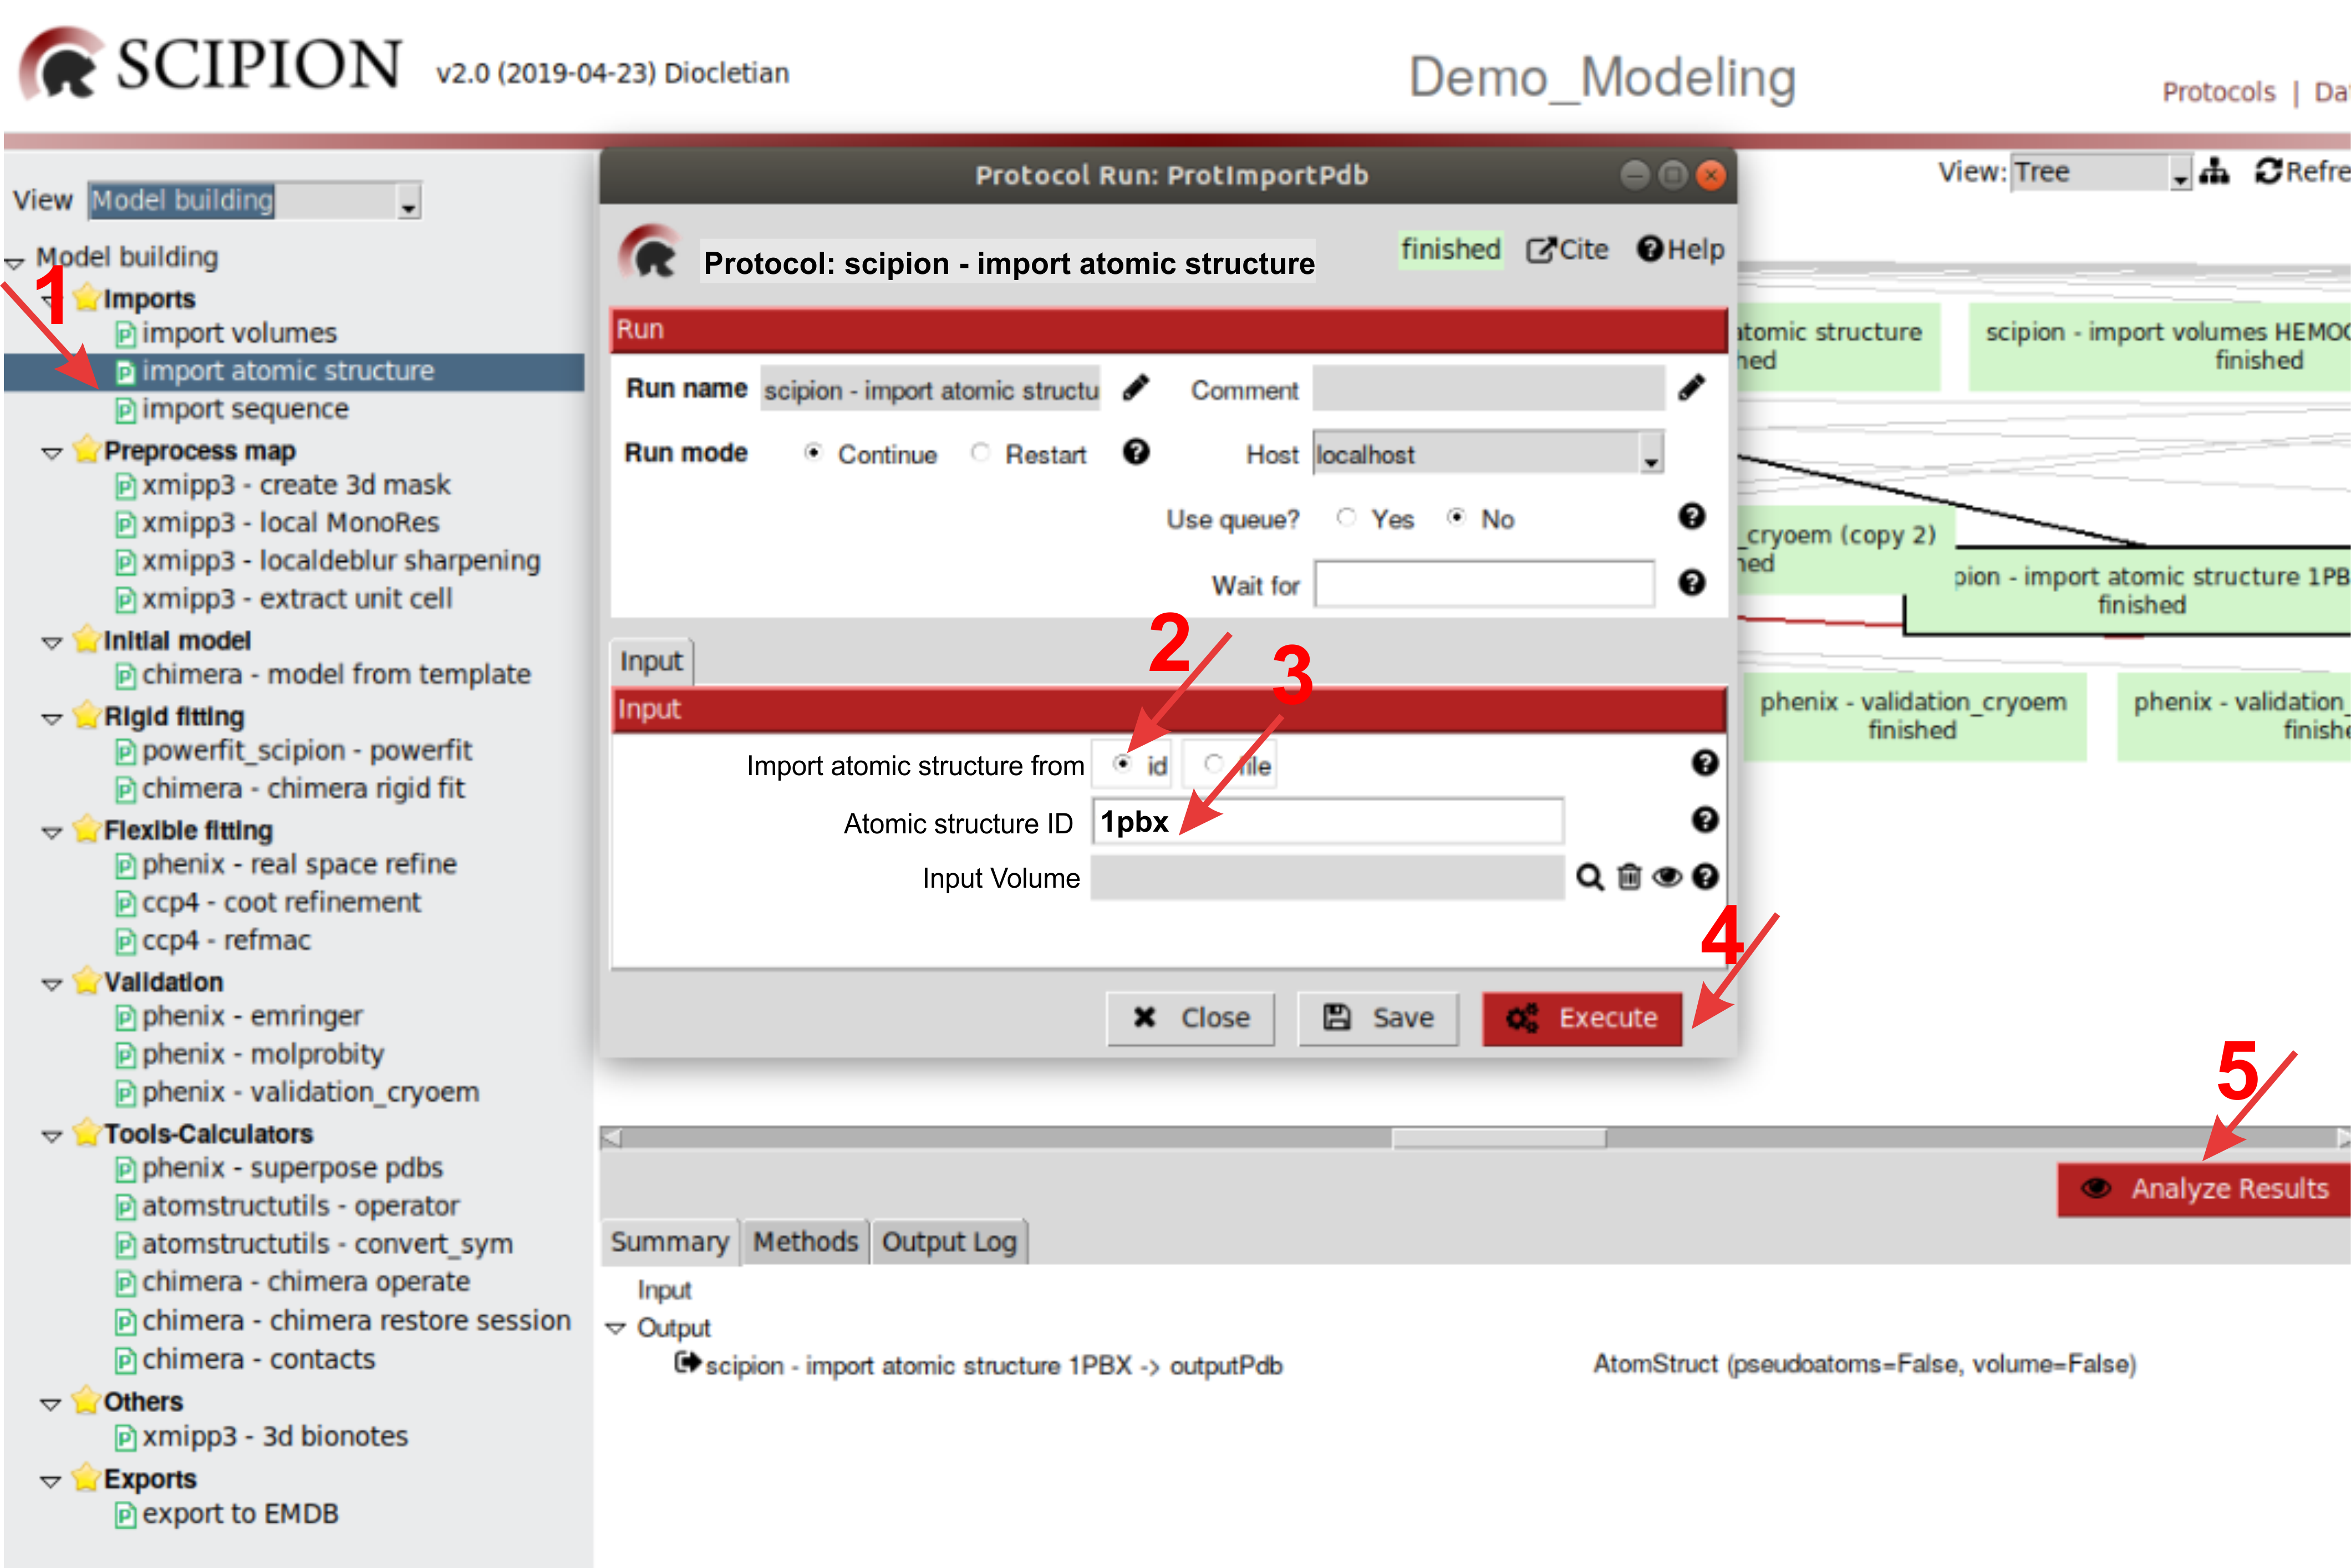
\includegraphics[width=0.90\textwidth]{Images/Fig10.png}
  \caption{Importing the atomic structure \ttt{1PBX}.}
  \label{fig:import_atomic_structure}
  \end{figure}
  
  \begin{figure}[H]
  \centering 
  \captionsetup{width=.7\linewidth} 
  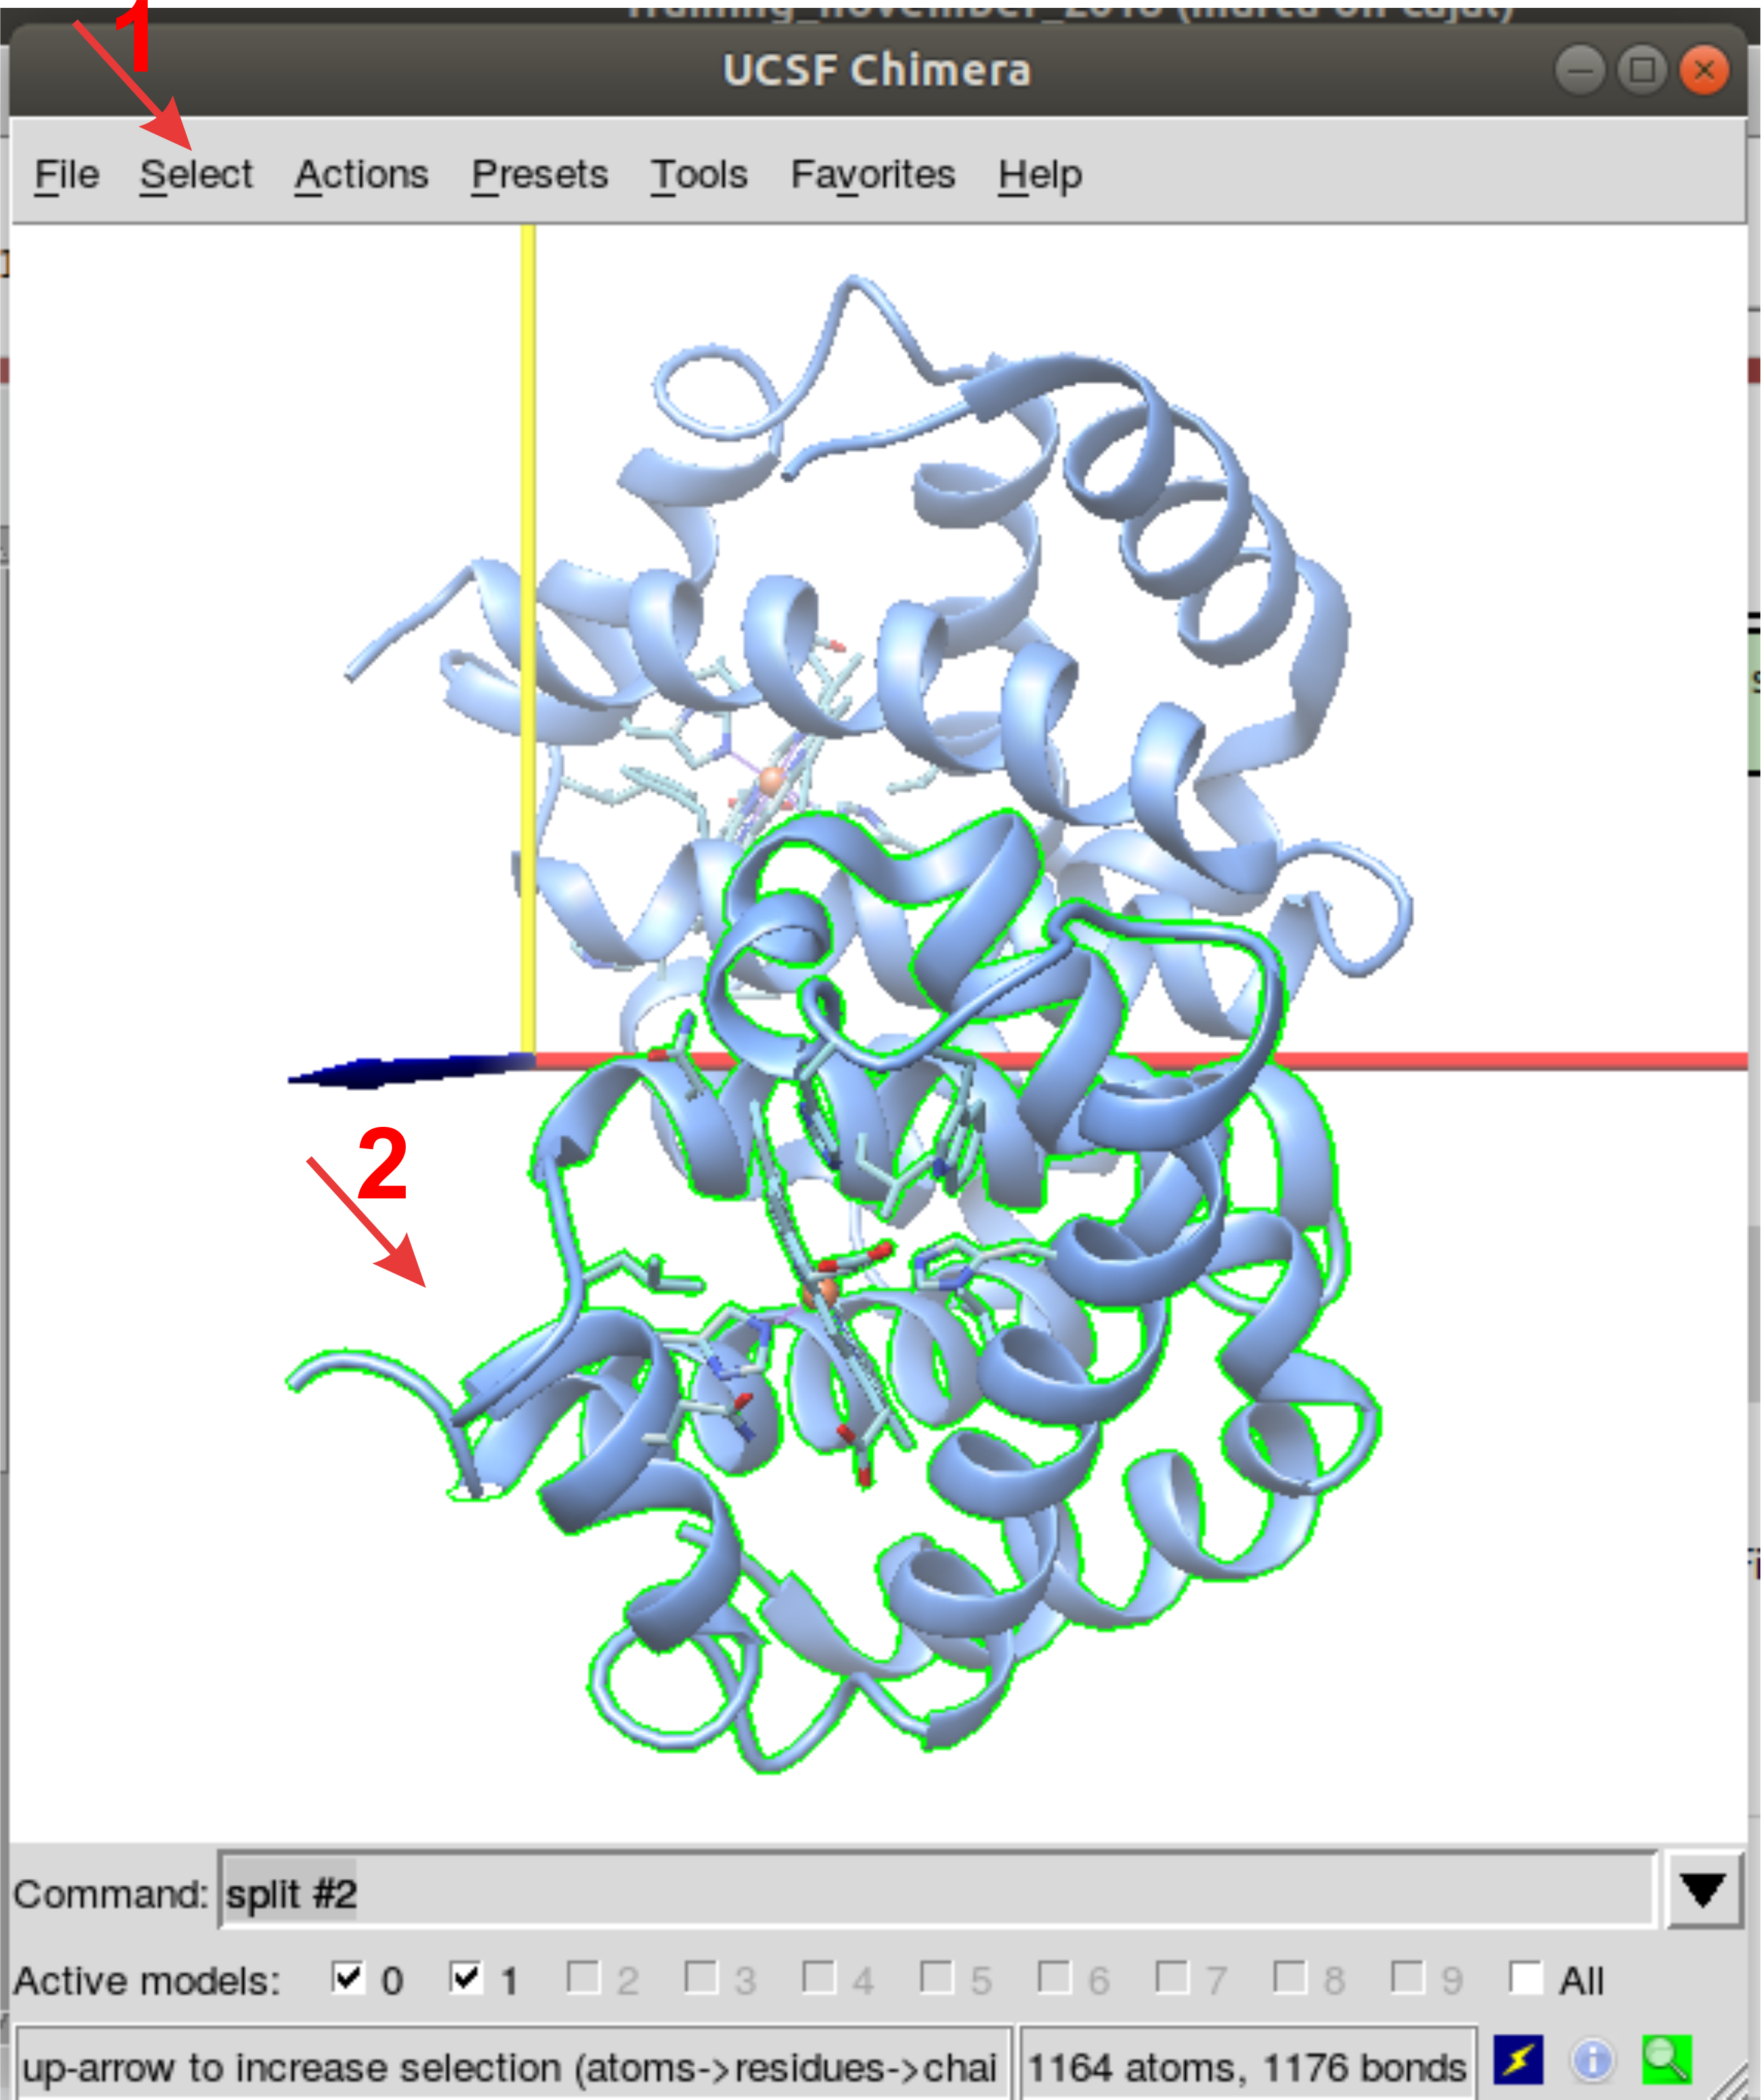
\includegraphics[width=0.50\textwidth]{Images/Fig11.png}
  \caption{Atomic structure \ttt{1PBX} visualized with Chimera. \ttt{Hgb} $\alpha$ subunit (chain \ttt{A}) is shown green-highlighted.}
  \label{fig:chimera_visualization_structure}
  \end{figure}
  
\subsubsection*{Structural models of human metHgb subunits from templates}

 $Modeller$ \citep{sali1993} is one of the computational web services used by $Chimera$, which provides the interface to run the program. Working with $Modeller$ requires a license key, which is provided free of charge for academic users. $Modeller$ allows two types of modeling computations to generate theoretical models, \iii{template}-based (sequence homology) and \iii{template}-free (\iii{de novo}, only for missing segments). In this tutorial we are going to consider the first one: structure prediction by sequence homology. Requirements for this type of modeling are the \iii{template} structure and a sequence alignment including sequences of \iii{target} and \iii{template}. 
 
 \begin{itemize}
 \item Preparing your sequence alignment:\\
In addition to the ways to obtain the \iii{target-template} sequence alignment using $Chimera$, this alignment can be also generated in the \scipion protocol \scommand{model from template} (Appendix \ref{app:modelFromTemplate}). This protocol allows selecting between pairwise and multiple sequence alignments. Besides producing more reliable alignments, especially for more distantly related sequences, multiple sequence alignments provide more structural information than pairwise alignments; they locate conserved regions in the molecule, thus improving predictions of structural arrangements due to mutant residues or residues that differ between \iii{template} and \iii{target} sequences \citep{pearson2013}. For this reason, in this tutorial we are going to perform a multiple sequence alignment. Additionally, you can also test the available tools to perform pairwise alignments.\\
 
Besides \iii{target} and \iii{template} sequence, some more sequences are needed to accomplish a multiple sequence alignment. The type and number of the sequences included depends on the sequence conservation, although they have to allow differentiating conserved regions. As an example, our multiple sequence alignment will include four more \ttt{Hgb} $\alpha$ subunit sequences from organisms located between human and fish in the evolutionary scale: \iii{Equus caballus} (Horse), \iii{Oryctolagus cuniculus} (Rabbit), \iii{Meleagris gallopavo} (Wild turkey), \iii{Aldabrachelys gigantea} (Aldabra giant tortoise). Download these sequences one by one from \ttt{UniProtKB} database filling in the \scommand{import sequence} protocol form with the appropriate accession codes (\ffigure{fig:multialignment_sequences}). A similar process has to be followed for \ttt{Hgb} $\beta$ subunit, importing \ttt{UniProtKB} sequences \ttt{P02062 (HBB\_HORSE), P02057(HBB\_RABIT), G1U9Q8 (G1U9Q8\_MELGA)} and \ttt{P83133 (HBB\_ALDGI)}.

  \begin{figure}[H]
  \centering 
  \captionsetup{width=.7\linewidth} 
  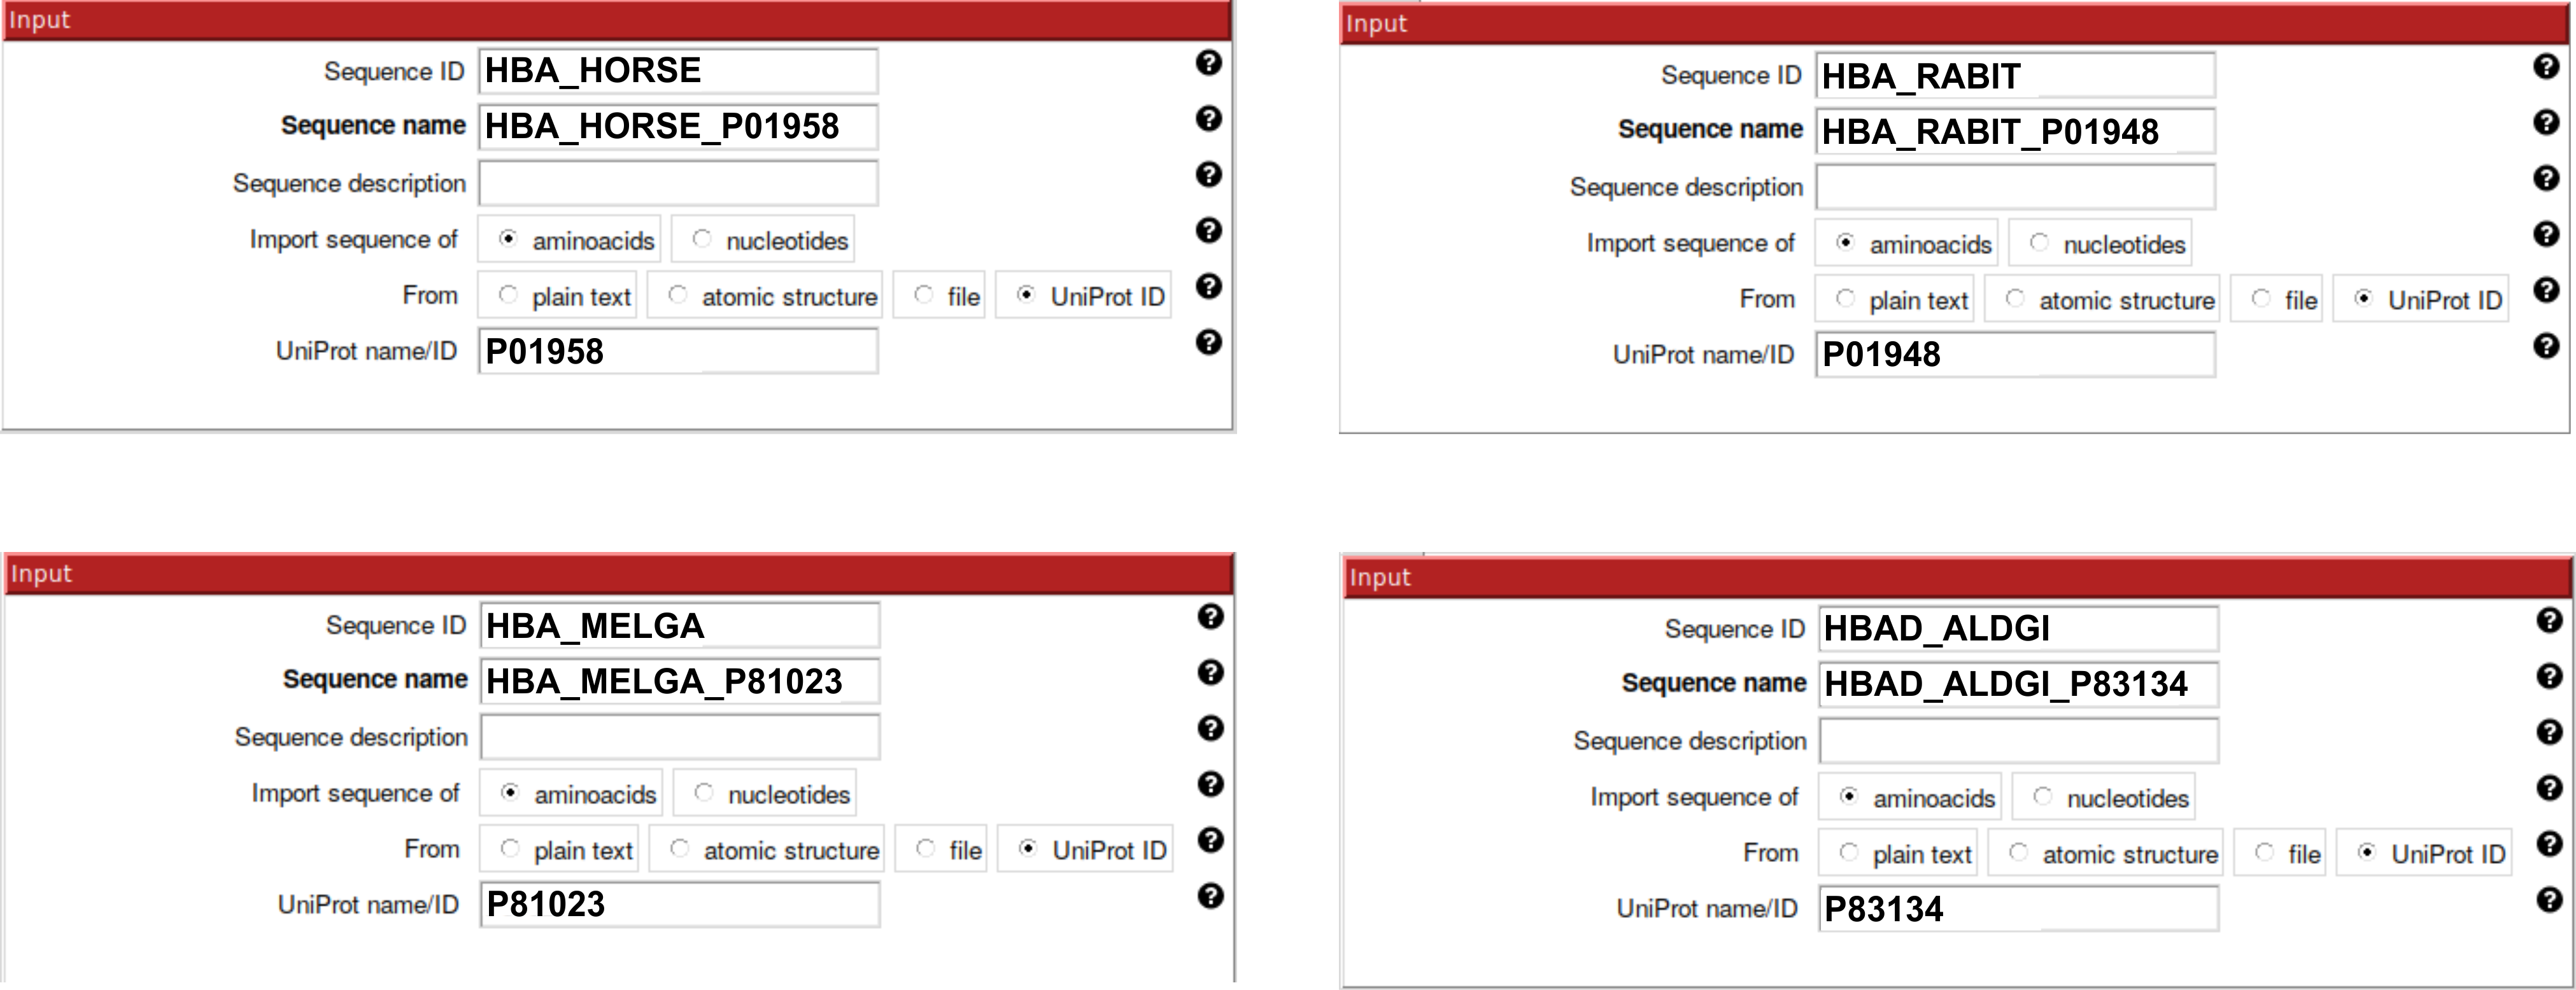
\includegraphics[width=0.95\textwidth]{Images/Fig12.png}
  \caption{Importing additional sequences to perform the multiple sequence alignment.}
  \label{fig:multialignment_sequences}
  \end{figure}

 \item Access to $Modeller$ in $Chimera$:\\
 The protocol \scommand{model from template} allows direct opening of the multiple sequence alignment in $Chimera$ and then, access to $Modeller$ via web service. Fill in the protocol form (\ffigure{fig:model_from_template_protocol} (1)), including the \iii{template} \ttt{1PBX} previously imported (2), the particular chain of interest (use the wizard to select it (3)) and the \iii{target} sequence of human \ttt{Hgb} $\alpha$ subunit (4). Since we plan to perform a multiple sequence alignment, we'd like to include additional sequences to align (5), that have to add next (6). Finally, select one of the multiple sequence alignment tools (7). 
 
 \begin{figure}[H]
  \centering 
  \captionsetup{width=.7\linewidth} 
  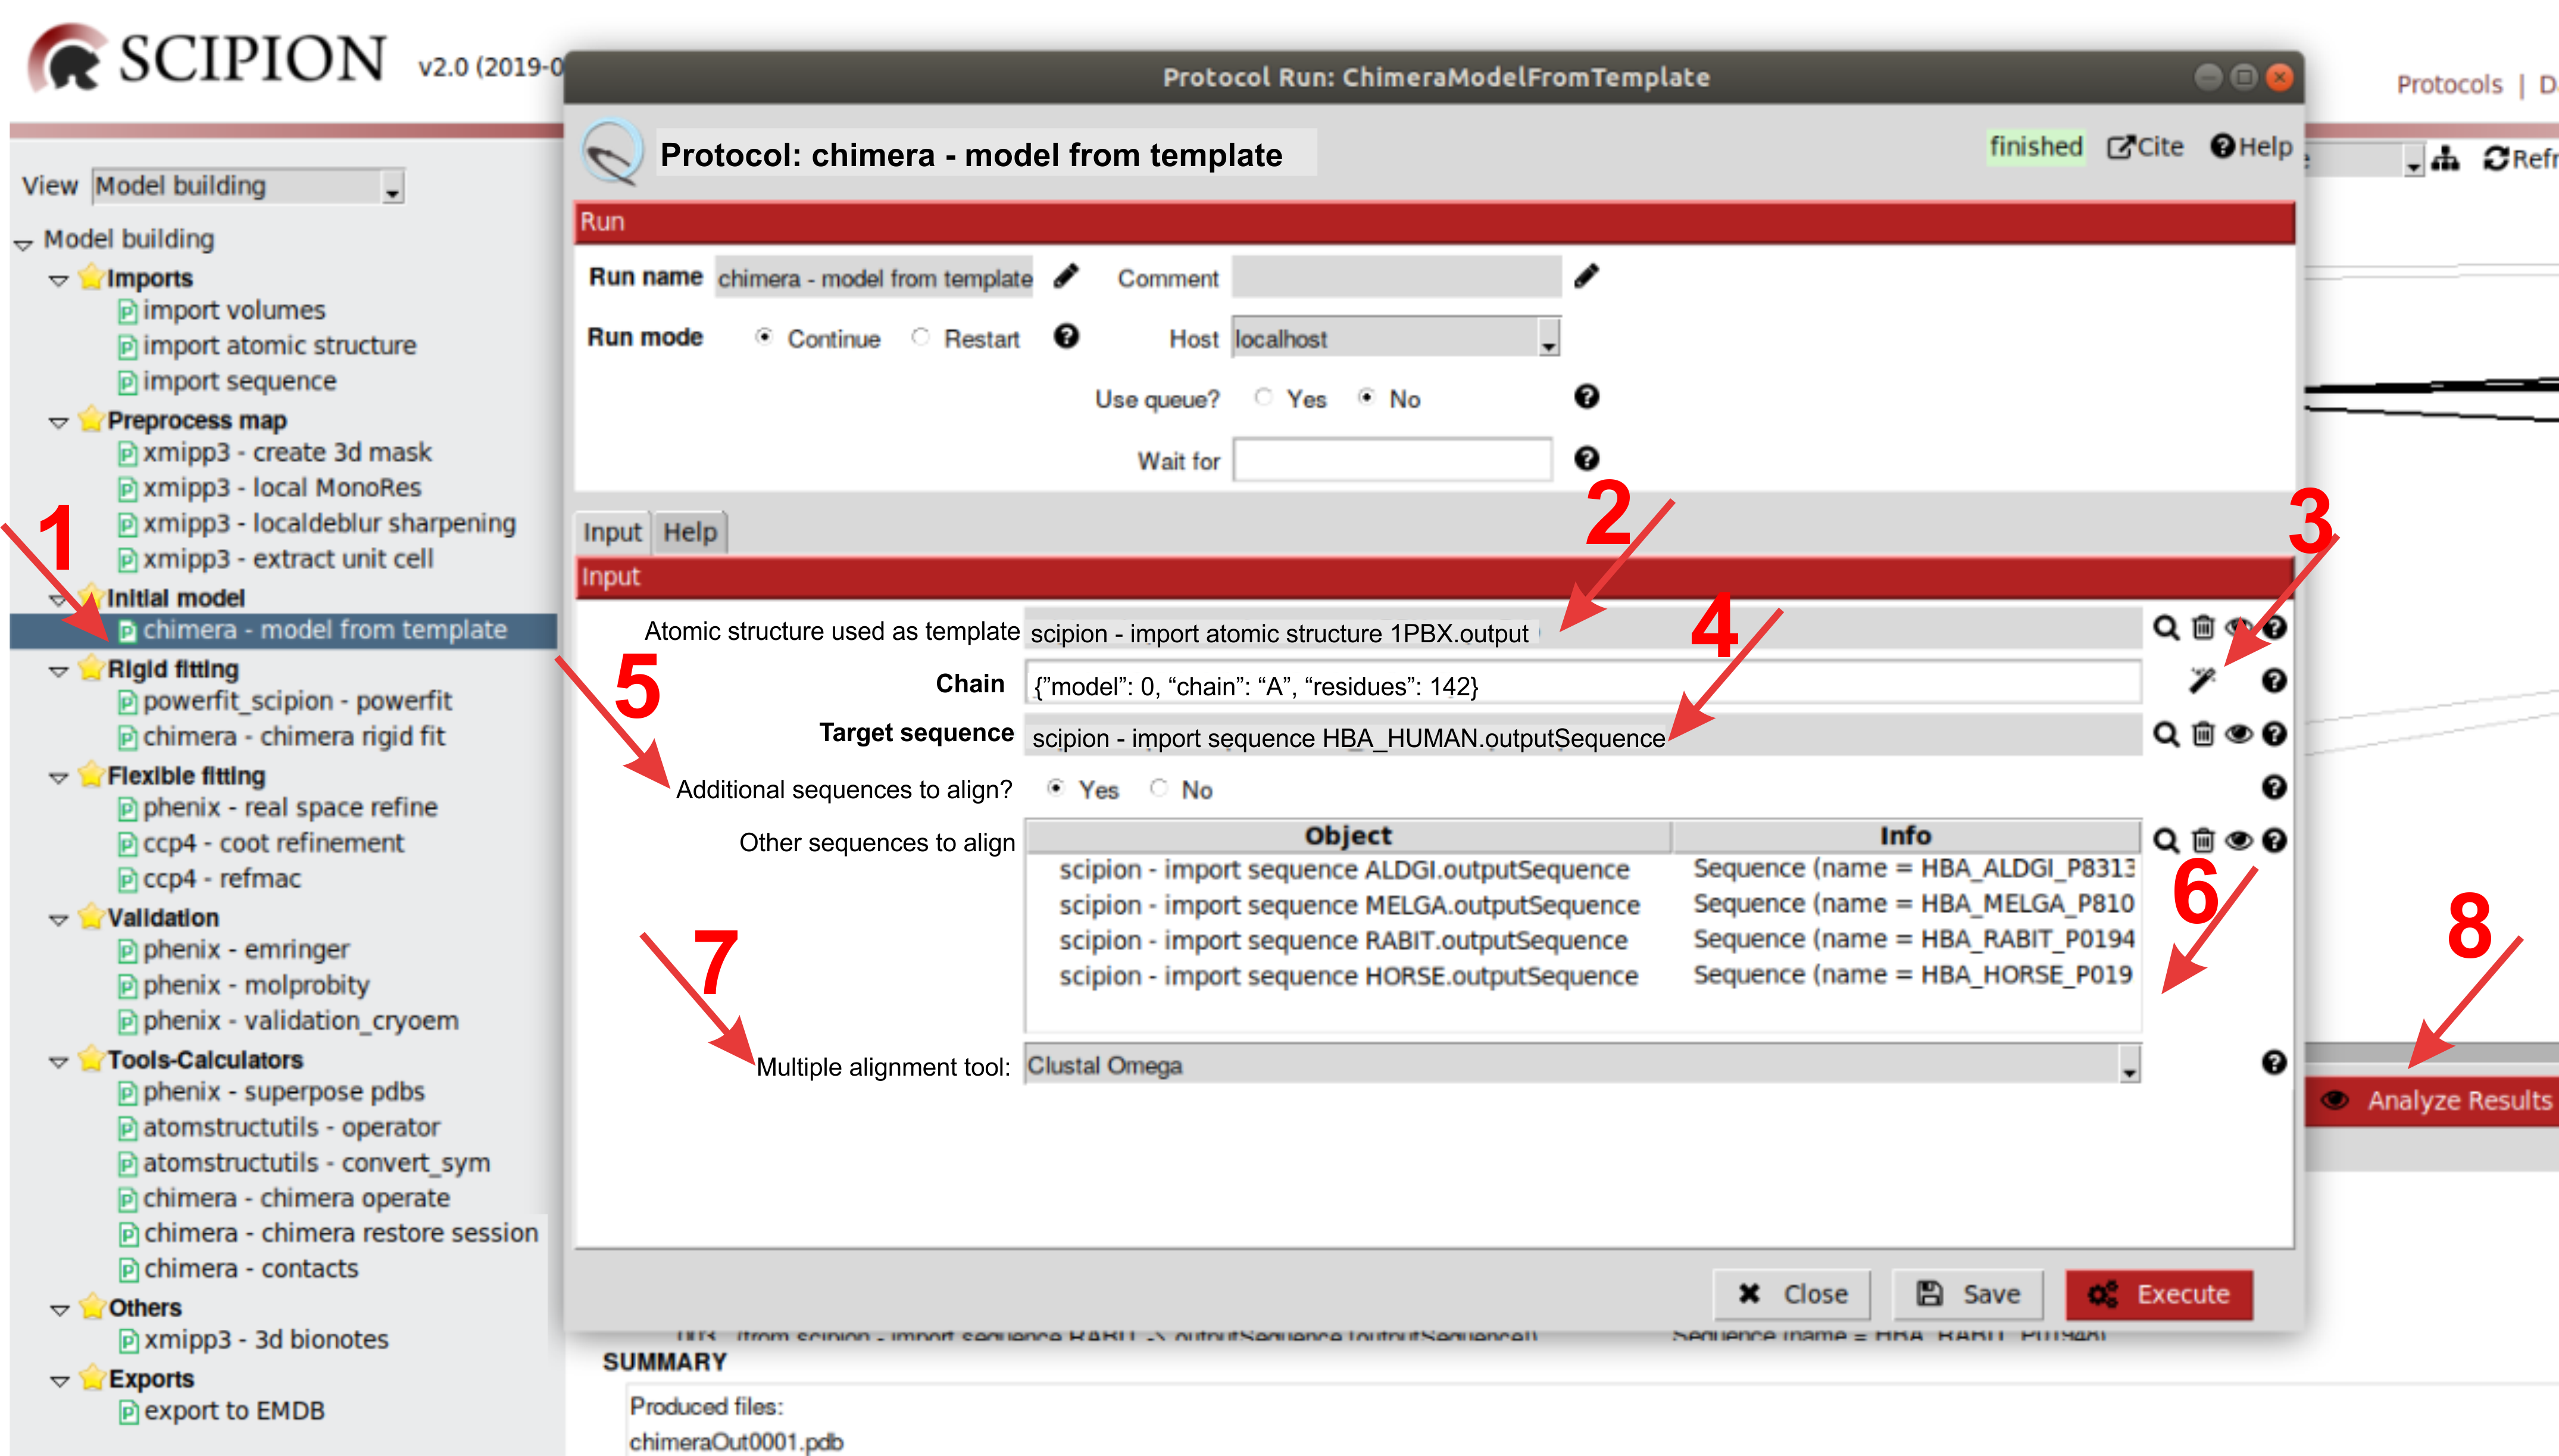
\includegraphics[width=0.90\textwidth]{Images/Fig13.png}
  \caption{Importing the multiple sequence alignment in $Chimera$.}
  \label{fig:model_from_template_protocol}
  \end{figure}
 
 A couple of windows will be open, the multiple sequence alignment in the upper part of \ffigure{fig:chimera_alignment}, and $Chimera$ graphics window. The \iii{template} selected chain is shown green-highlighted in both windows. As you may observe in the alignment, \ttt{Hgb} $\alpha$ subunit is a quite conserved macromolecule; there is only one gap in the alignment because \ttt{PRO} (Proline) 47 residue has disappeared during evolution. Human \ttt{Hgb} $\alpha$ subunit is closer to the protein in mammals (horse, rabbit) than to the protein in unrelated organisms, as we would have anticipated. Corroborate this point by checking the identity percentage \%ID  between human sequence and the other sequences in \ffigure{fig:modeller} (B). 
 
 \begin{figure}[H]
  \centering 
  \captionsetup{width=.7\linewidth} 
  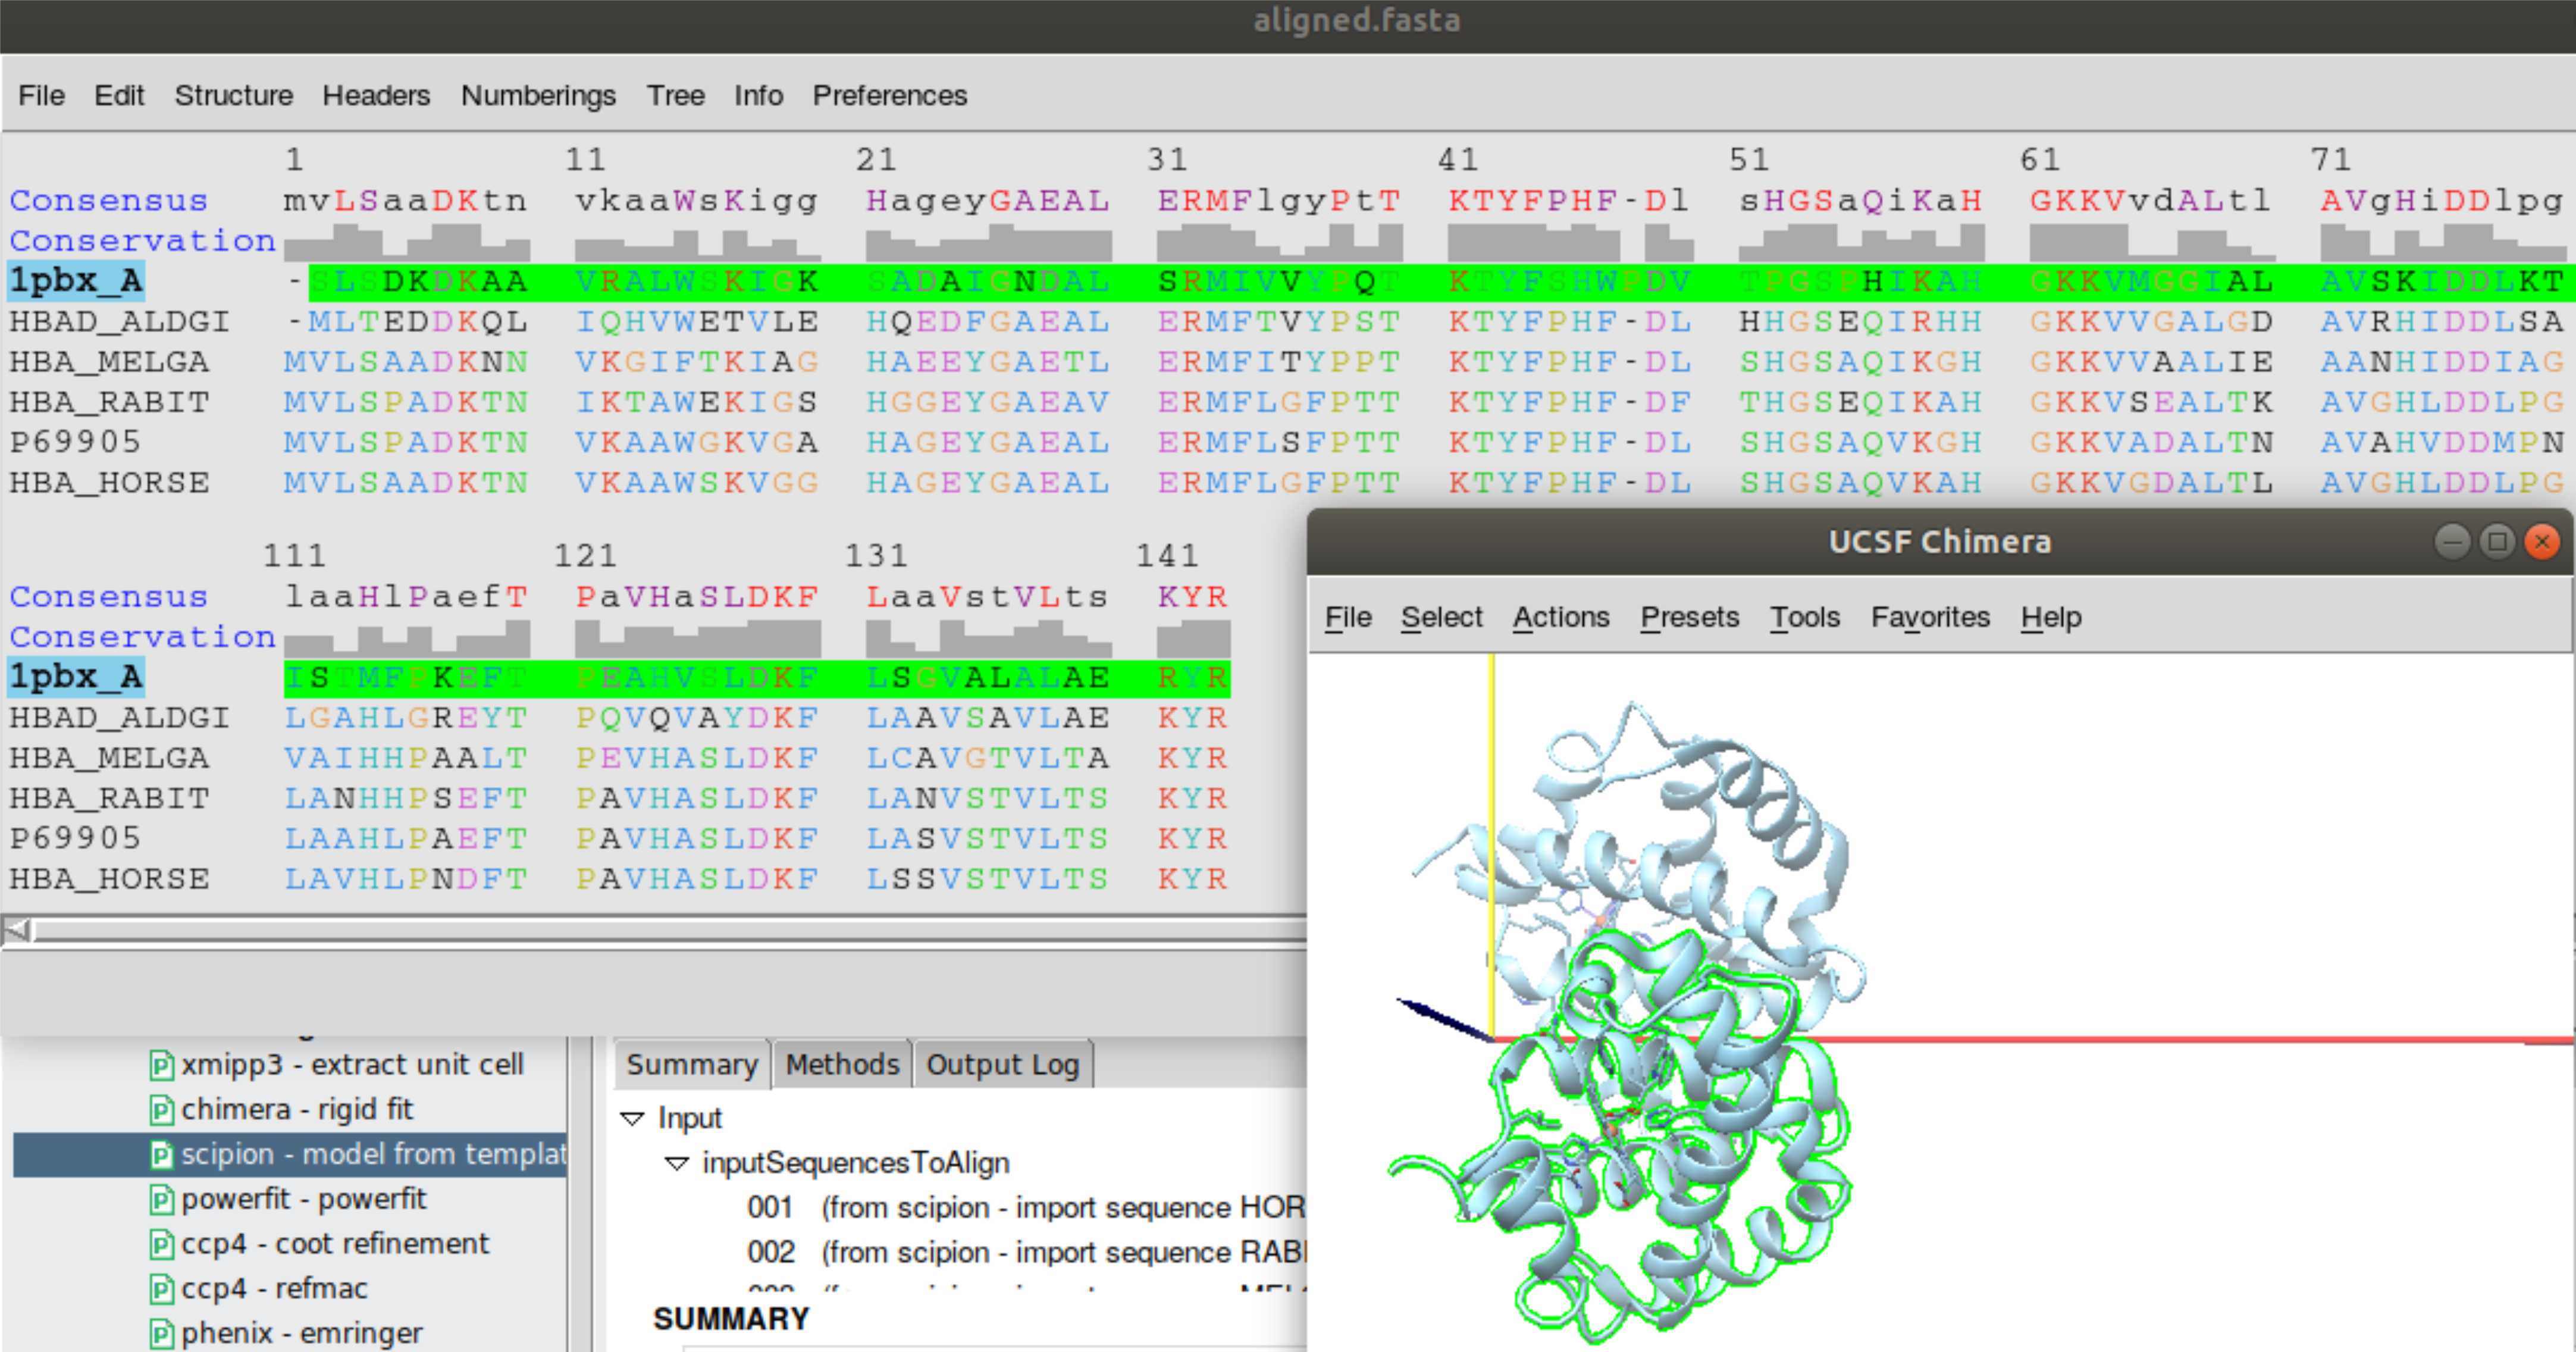
\includegraphics[width=0.80\textwidth]{Images/Fig14.png}
  \caption{Opening the multiple sequence alignment in $Chimera$.}
  \label{fig:chimera_alignment}
  \end{figure}
\end{itemize}

In case you'd like edit the name or the order of the sequences, add,  delete or realign sequences, ..., go to the upper menu of the multiple sequence alignment (\ttt{Edit -> }). In particular, we are going to change the name of the \iii{target} sequence from \ttt{P69905} to \ttt{HBA\_HUMAN} in \ttt{Edit -> Edit Sequence Name...} (\ffigure{fig:modeller} (A)). To get possible atomic models of the \iii{target} sequence in $Modeller$ web service, we have to select \ttt{Structure -> Modeller (homology ...)} in the same upper menu. A new window for Comparative Modeling with Modeller will be open (\ffigure{fig:modeller} (B)), that we have to fill in selecting \iii{target} sequence (1) and \iii{template} (2). Modeller license key has to be included here (3). The number of output models can be specified in Advanced Options (5 by default). Finally, press Apply to start the computation without hide the panel (4) or OK to start the computation hiding it. In $Chimera$ main graphics window, lower left corner, you may see the status of your job. After a while, five possible atomic structures, from now ahead \iii{models}, are retrieved for the \iii{target} sequence (\ffigure{fig:modeller} (C)) together with their assessment scores. Column \ttt{GA341} of Modeller Results indicates the score derived from statistical potentials (values in \ttt{[0,1]}; \ttt{> 0.7} for reliable \iii{models}). Column \ttt{zDOPE} (normalized Discrete Optimized Protein Energy) score depends on the atomic distance (negative values for the better \iii{models}). Let's select \iii{model} \ttt{\#2.1}. You can check every model numbers in $Chimera$'s main menu (\ttt{Favorites -> Model Panel}).
 
  \begin{figure}[H]
  \centering 
  \captionsetup{width=.7\linewidth} 
  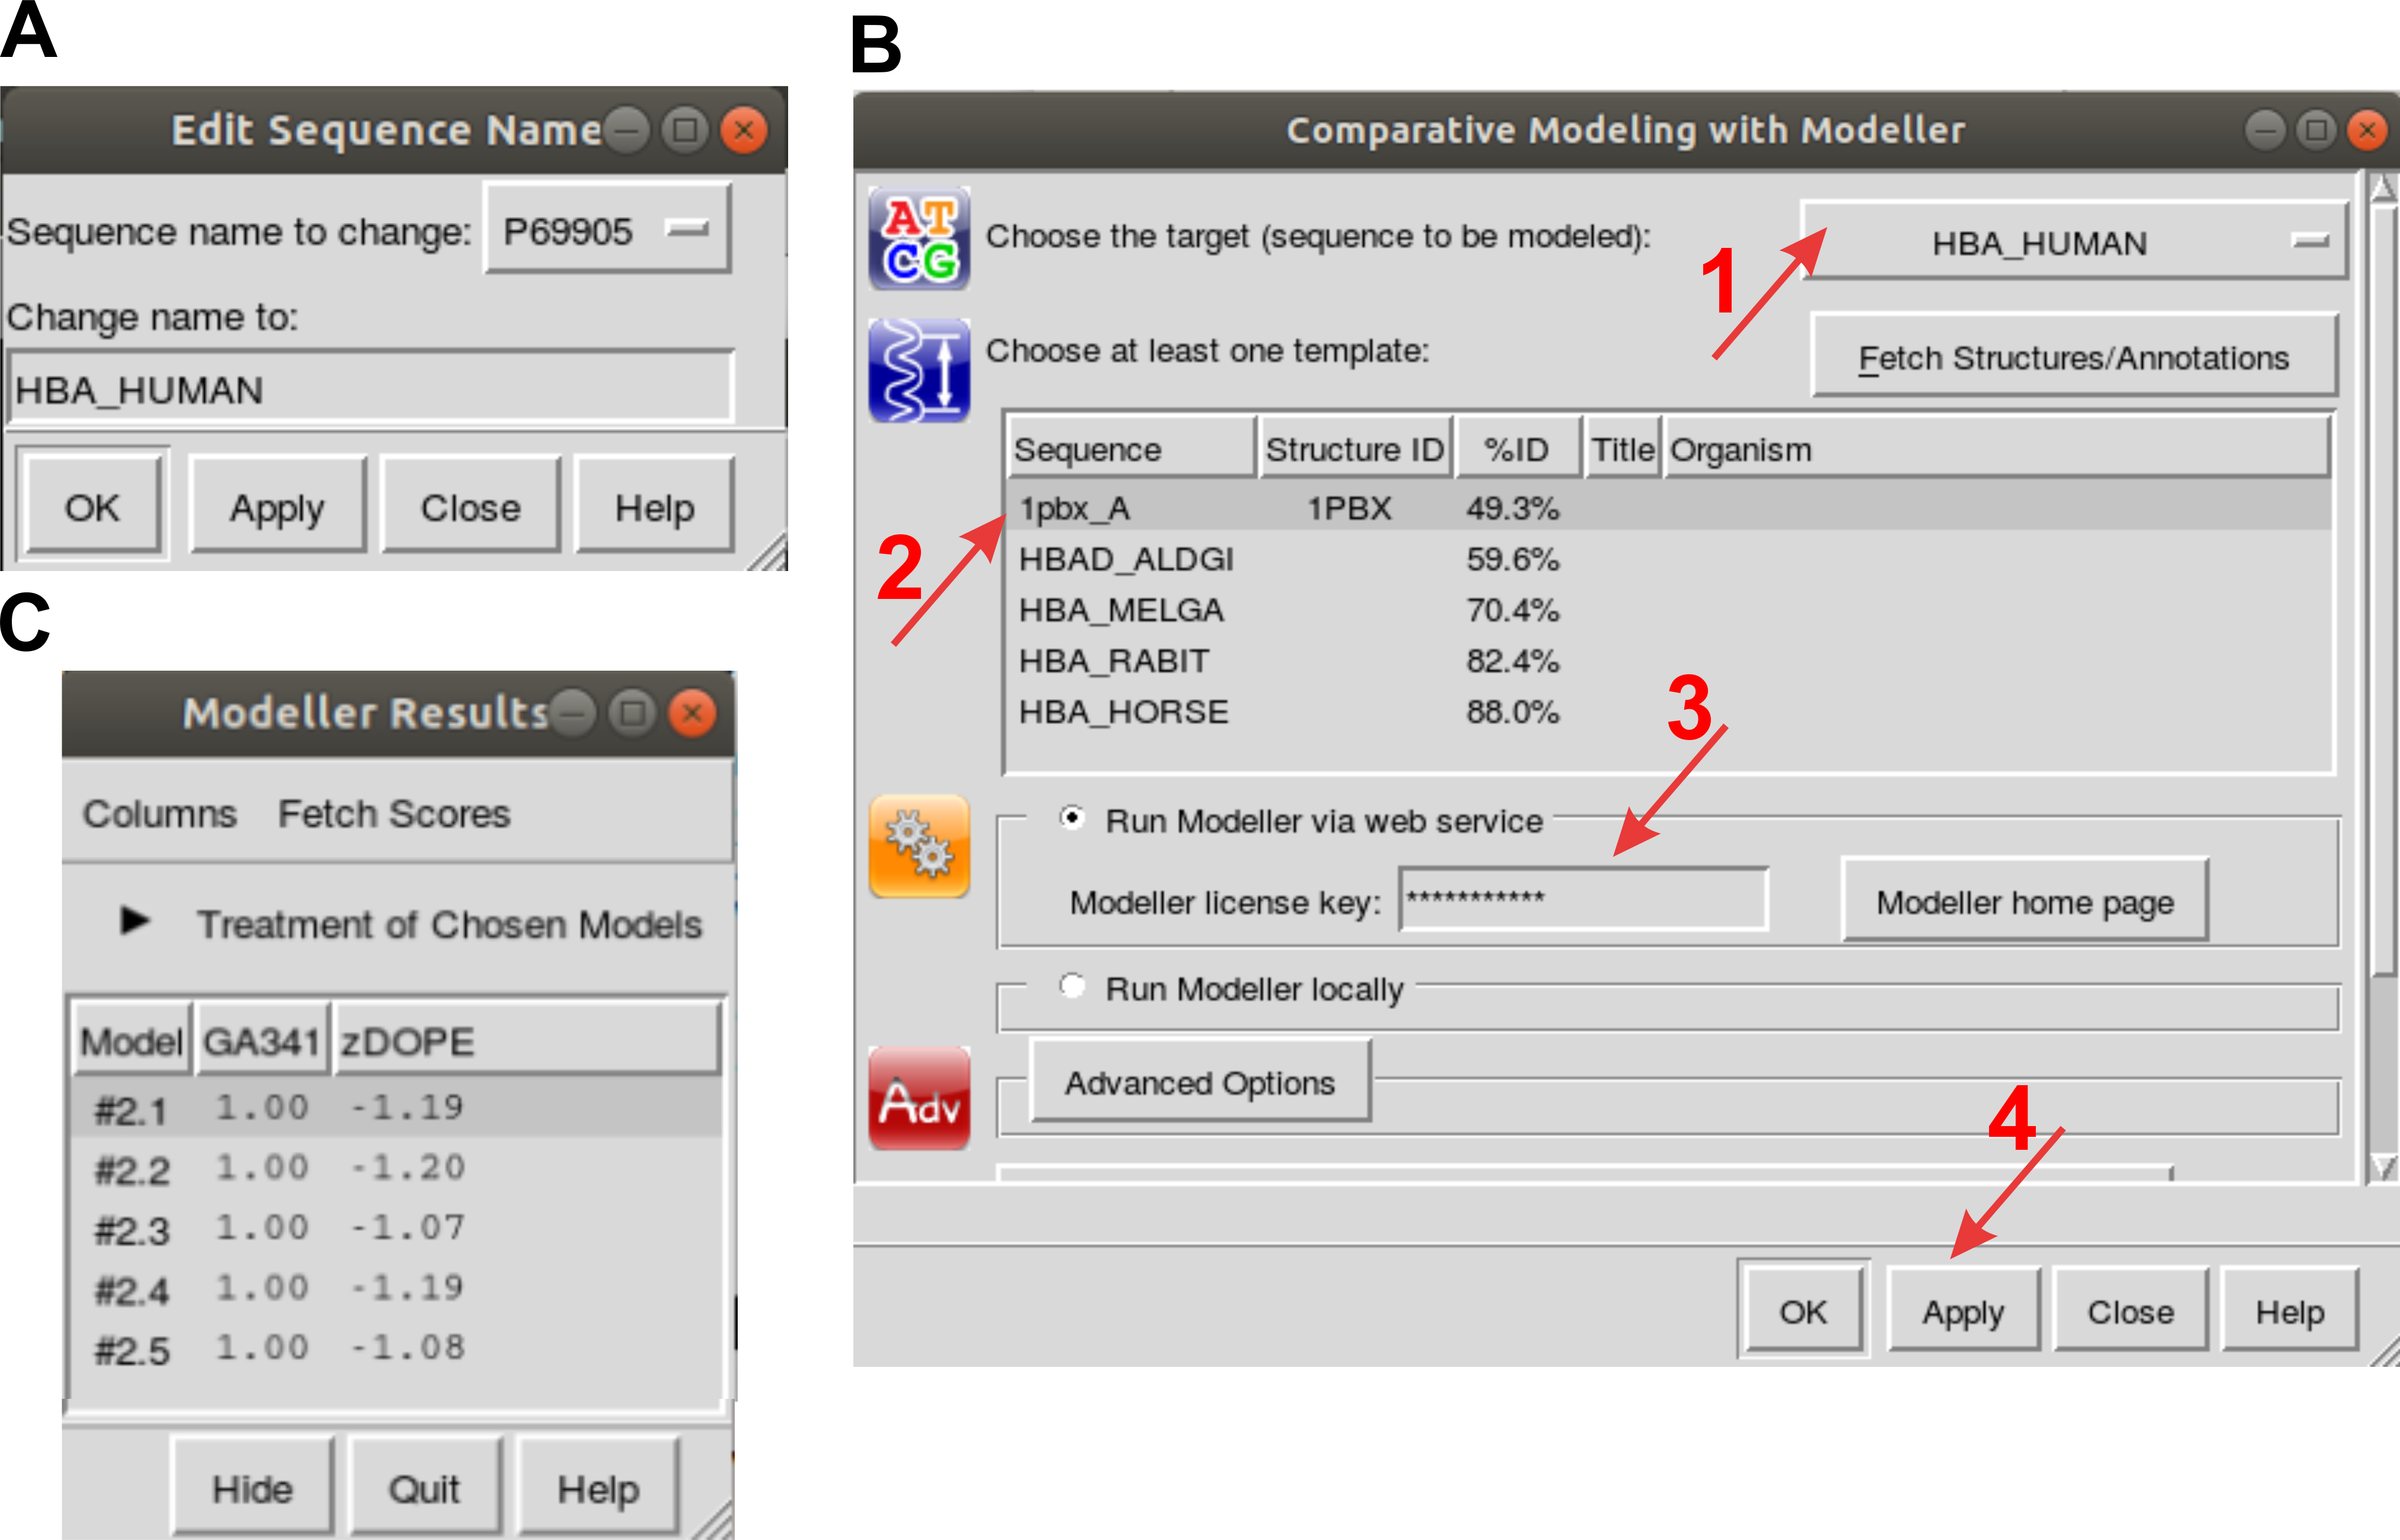
\includegraphics[width=0.80\textwidth]{Images/Fig15.png}
  \caption{(A) Sequence edition. (B) Completing the form to access to homology modeling with $Modeller$. (C) Resulting \iii{models}.}
  \label{fig:modeller}
  \end{figure}
 
 Comparing your selected \iii{model} of human \ttt{metHgb} $\alpha$ subunit with \ttt{1PBX\_A} \iii{template}, we observe that the selected \iii{model} \ttt{\#2.1} does not contain the \ttt{HEME} prosthetic group (\ffigure{fig:chimera_model} (A)). Before saving the \iii{model}, the \iii{template} \ttt{HEME} group will thus be added to your \iii{model} in $Chimera$. With this aim, open $Chimera$'s command line; from $Chimera$ main menu (\ttt{Favorites -> Command Line}) and delete every atom of \ttt{1PBX} \iii{template}, except the \ttt{HEME} group associated to chain \ttt{A}. To preserve residue 144 (\ttt{HEME} group) in chain \ttt{A}, write the next command line (\ffigure{fig:chimera_model} (A)(1)):\\ 
 
 \ttt{delete \#1:0-143.A, 145-.A, .B}\\ or\\
 \ttt{delete \#1:0-143.A}\\ \ttt{delete \#1:145-.A}\\ \ttt{delete\#1:.B}\\
 
 Go to the Model Panel and select models \ttt{\#1} and \ttt{\#2.1} simultaneously, then press \ttt{Copy/Combine} on the right side column (\ffigure{fig:chimera_model} (B)(2)). Model Panel shows the new \iii{model} created \ttt{\#3} (3), that we can save in the command line (4) writing:\\
 
 \ttt{scipionwrite model \#3}\\
 
 \begin{figure}[H]
  \centering 
  \captionsetup{width=.7\linewidth} 
  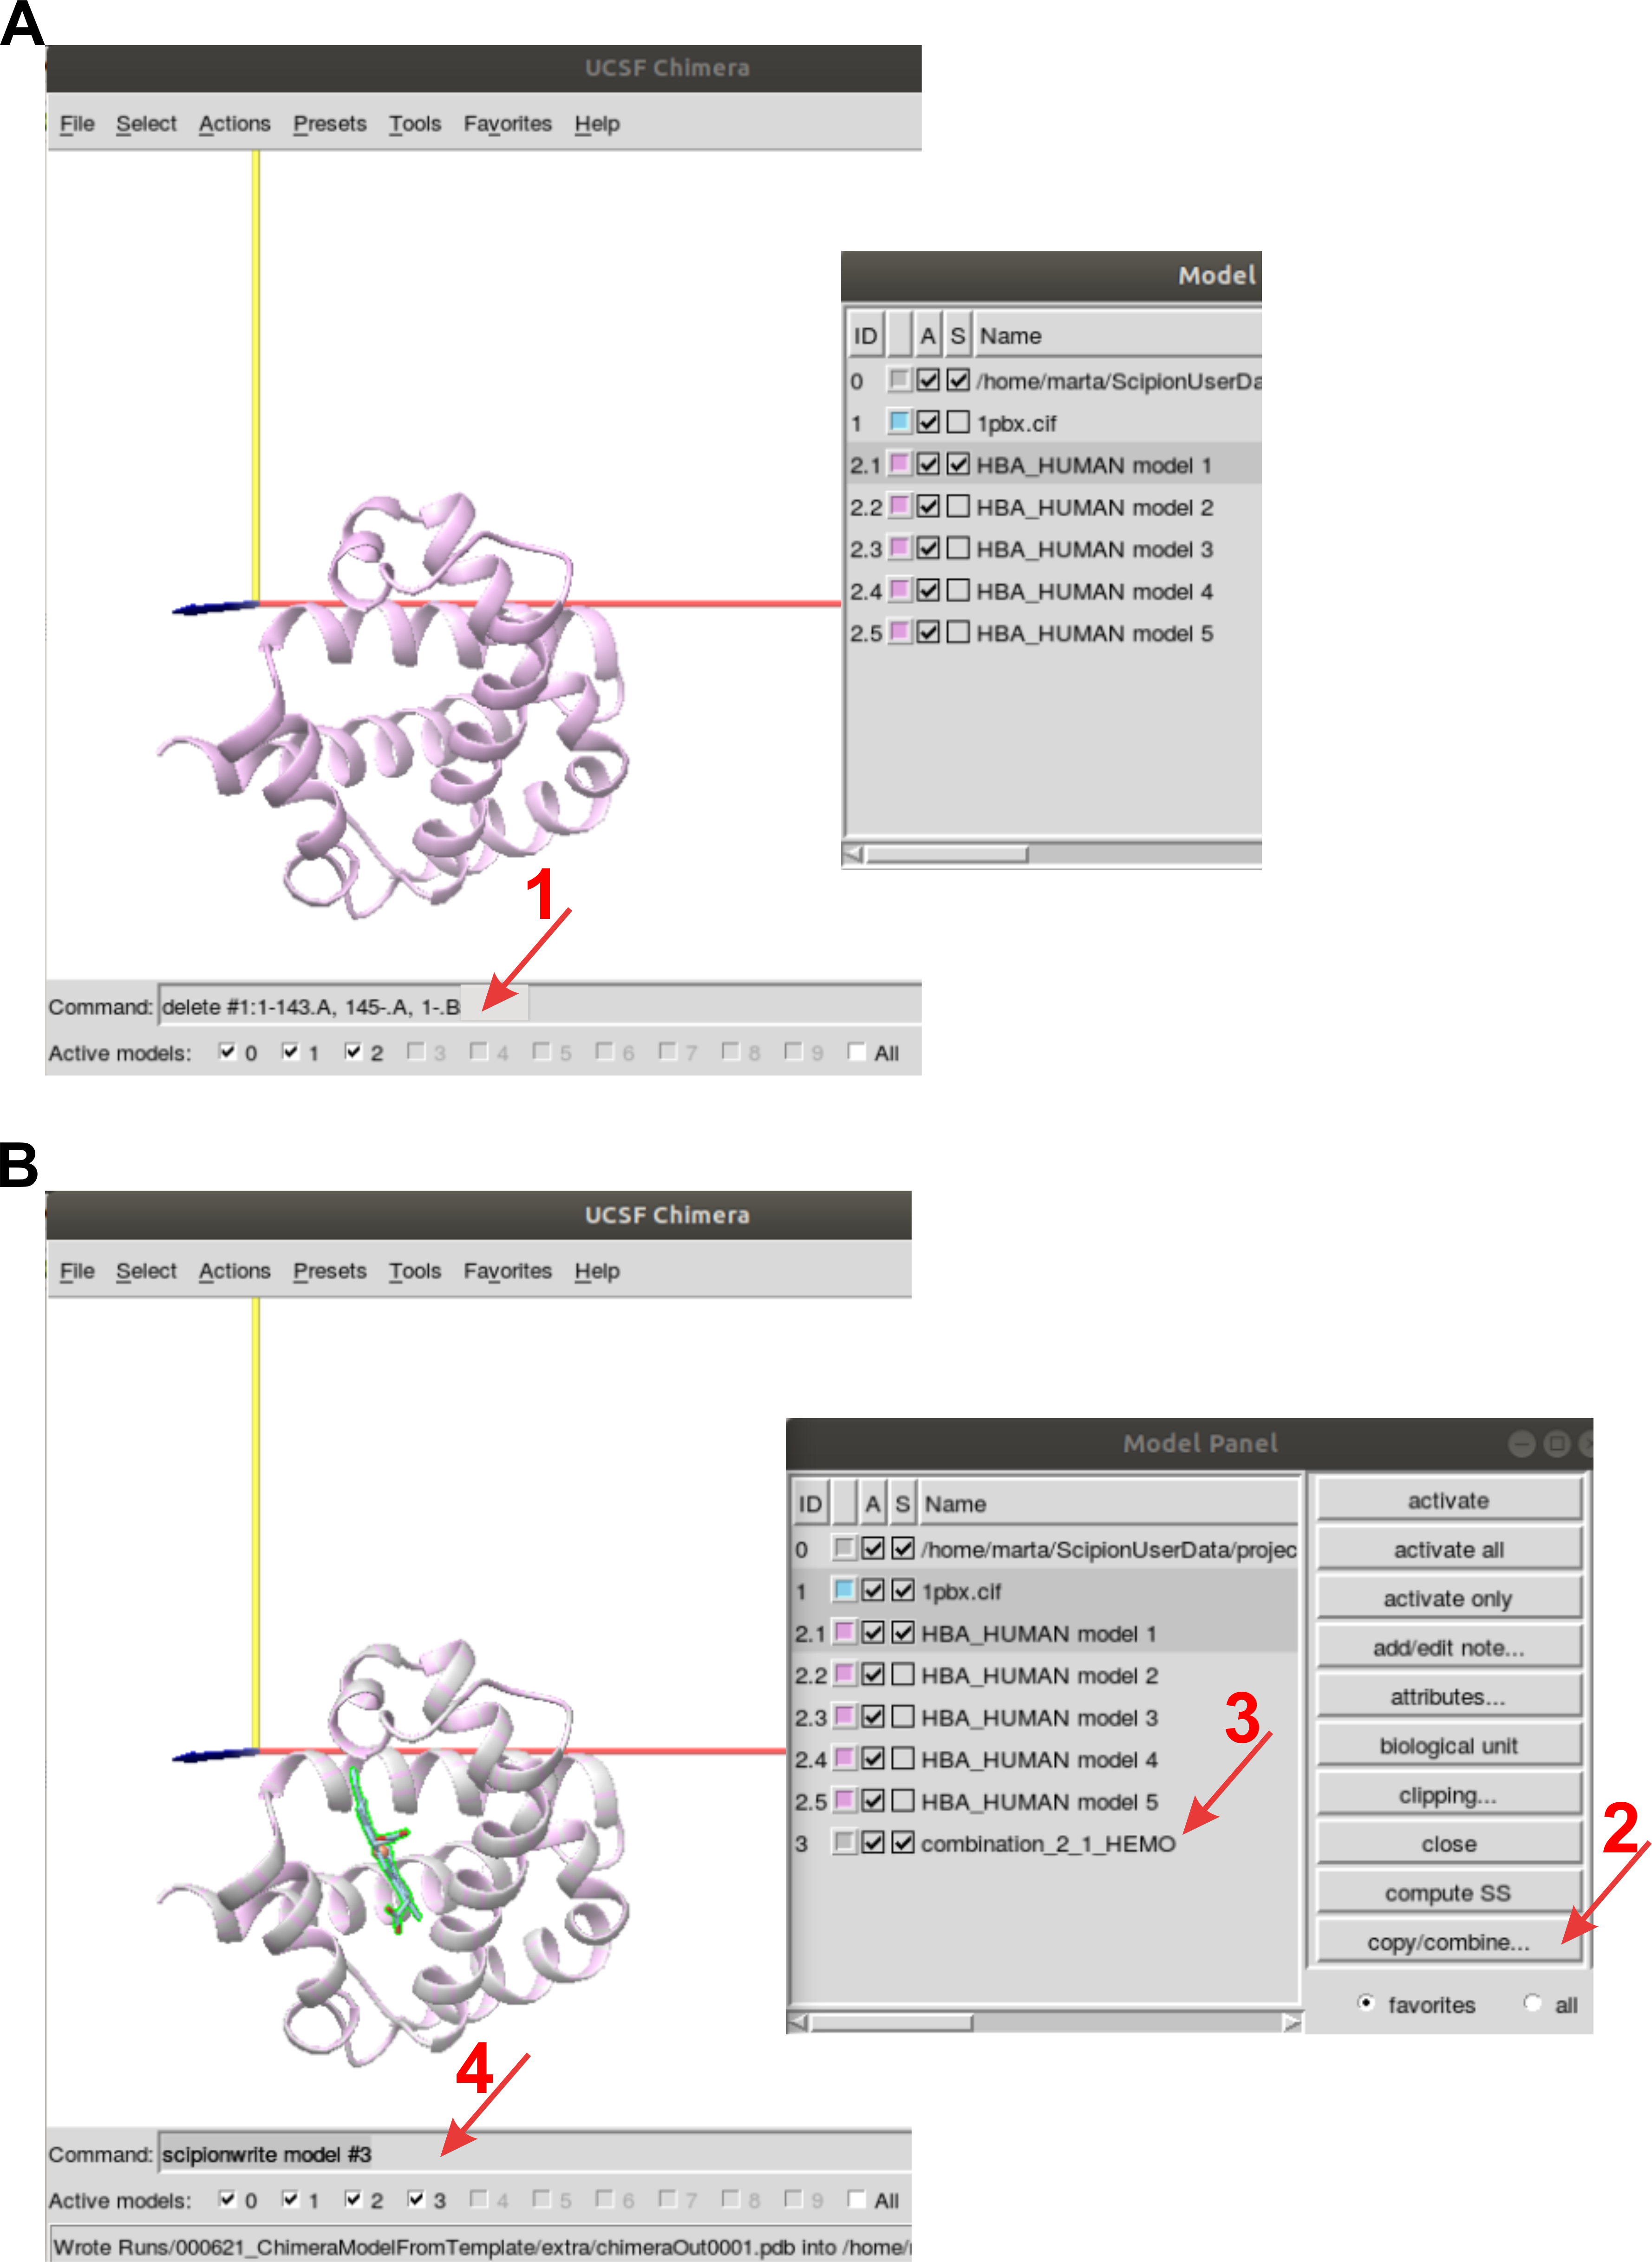
\includegraphics[width=0.80\textwidth]{Images/Fig16.png}
  \caption{\iii{Model} selection in $Chimera$. (A) Selected \iii{model} \ttt{\#2.1}. (B) Creation of full final \iii{model} of human \ttt{metHgb} $\alpha$ subunit, including \ttt{HEME} group.}
  \label{fig:chimera_model}
  \end{figure}
 
 After closing $Chimera$, you can visualize (\ffigure{fig:model_from_template_protocol} (8)) your full predicted \iii{model}. In a similar process, you can also obtain human \ttt{metHgb} $\beta$ subunit. Remark that in this case, the \ttt{HEME} group will be kept with the next $Chimera$ command line: \\
 \ttt{delete \#1:.A, 0-147.B, 149-.B}\\ or \\
 \ttt{delete \#1:.A}\\ \ttt{delete \#1:0-147.B}\\ \ttt{delete \#1:149-.B}\\
  
If for any reason you decide to go back and check a different \iii{model} from the five \iii{models} initially provided by $Modeller$, you can do it by using \scommand{chimera restore session} protocol (Appendix \ref{app:chimeraRestoreSession}). This protocol is allowed to be used whenever $Chimera$ session had been saved, specifically after using protocols $Chimera$ \ttt{rigid fit}, $Chimera$ \ttt{operate}, and \scipion \ttt{model from template}. In addition to the $Chimera$ command line \ttt{scipionss}, command line \ttt{scipionwrite} also save $Chimera$ session by default. So, if you want to restore a previous session just open the form (\ffigure{fig:restore_session_protocol}, 1), and include the session that you'd like to restore (2).

 \begin{figure}[H]
  \centering 
  \captionsetup{width=.7\linewidth} 
  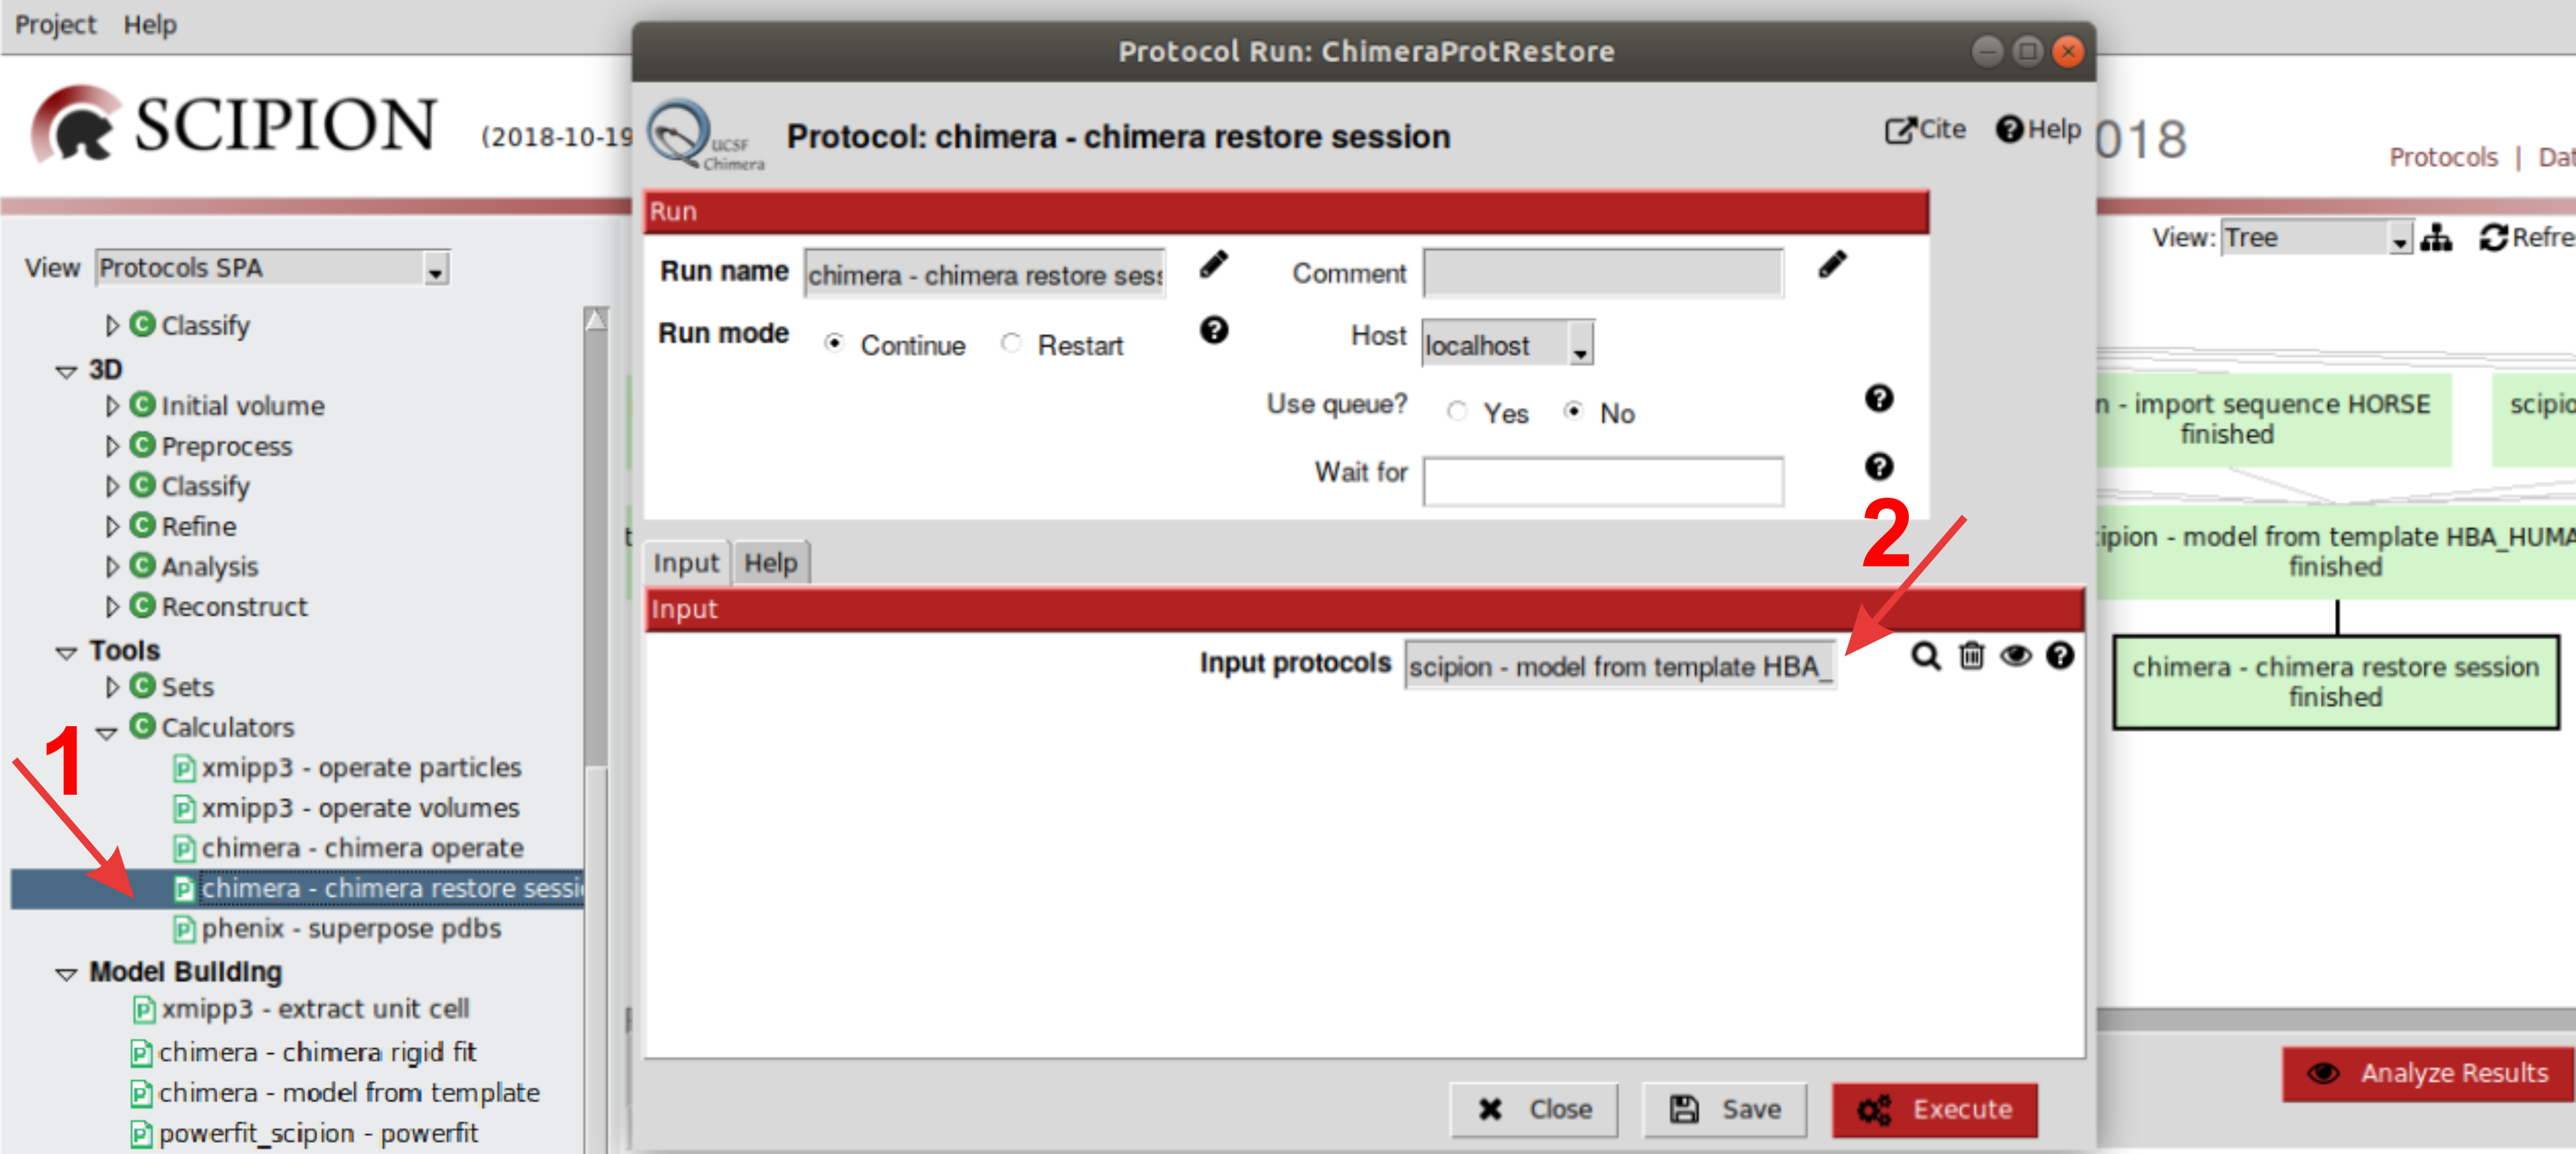
\includegraphics[width=0.90\textwidth]{Images/Fig17.png}
  \caption{Restoring session in $Chimera$.}
  \label{fig:restore_session_protocol}
  \end{figure}
